Ein Schaltkreis wie in Abbildung \ref{fig:Abb6} dargestellt ist die Grundlage für alle Messungen. Die Als erstes müssen die Frequenzen der beiden Schwingkreise aufeinander abgestimmt werden, da eine der Kapazitäten variabel ist. \\
\begin{figure}[h!]
	\centering
	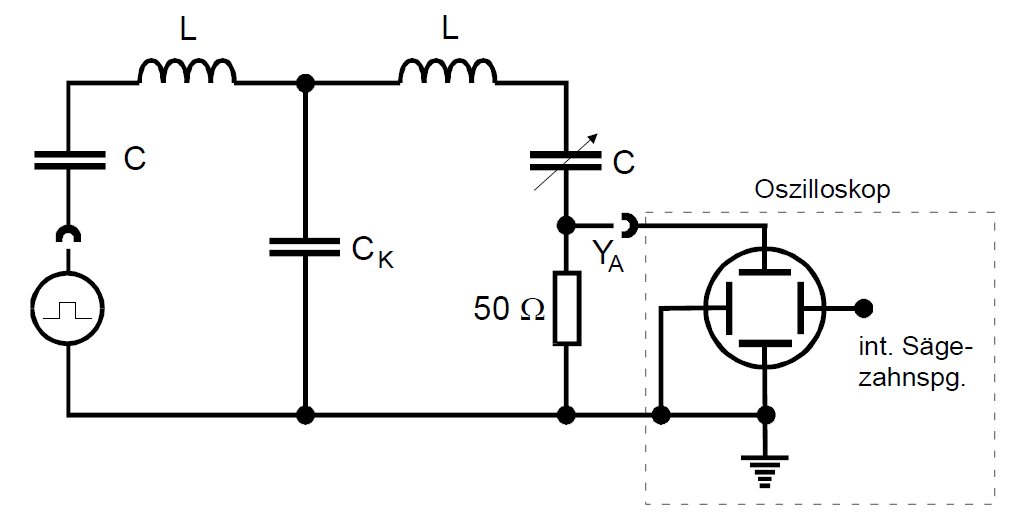
\includegraphics[width=0.7\textwidth]{Abb6.png}
	\caption{Schaltkreis für alle Messungen}
	\label{fig:Abb6}
\end{figure}
Die Frequenzen der Fundamentalschwingungen werden auf zwei Methoden bestimmt. Zuerst wird der Erreger durch eine Sinusspannung ersetzt und mit Hilfe von Lissajous-Figuren festgestellt, für welche Frequenzen bei Variation der Erregerfrequenz beide Schwingkreise um die Phasen 0 und $\pi$ verschoben sind. Bei der zweiten Methode erzeugt man ein kontinuierliches Frequenzspektrum und zeichnet den Stromverlauf des rechten Schwingkreises über die Zeit auf. Wenn der Strom ein Maximum einnimmt, ist die Frequenz gerade $\nu^+$ oder $\nu^-$. \\
Des Weiteren wird die Schwebung untersucht, indem einer der beiden Schwingkreise mit einem einzelnen Impuls (bzw. Rechteckimpuls mit einer viel kleinerer Frequenz als der Schwing- und Schwegunsfrequenz) angeregt wird. Es sollen die Maxima der Schwingung innerhalb einer Schwebungsperiode für verschiedene Kapazitäten des Kondensators $C_\text{K}$ auf einem Oszilloskop beobachtet werden.
\subsubsection*{Kenndaten der Bauteile \label{sec:Bauteile}}
Die Induktivität der verwendeten Spulen ist
\[ L = \SI{23.954}{\milli\henry} \ . \]
Die Kondensatoren in den Schwingkreisen haben eine Kapazität von
\[ C^* = \SI{0.7932}{\nano\farad} \ . \]
Es gilt zu beachten, dass auch die Spulen eine Kapazität von
\[ C_\text{Sp} = \SI{0.028}{\nano\farad} \]
haben. Das erschwert die Rechnung kaum, da mit
\[ C = C^* + C_\text{Sp} \]
gerechnet werden kann. \\